%!TEX root = cvl_bachelor_thesis.tex

%----------------------------------------------
% Related Work
%----------------------------------------------
\section{Related Work}
\label{sec:relatedWork}
Software für die Bildsuche in radiologischen Daten gibt es bis jetzt noch nicht,  
allerdings decken sich die Anforderungen großteils mit Betrachtungstools für 2D und 3D Daten aus der Radiologie und Nuklearmedizin.
Solche Softwareprodukte finden sich in den Betrachtungs-Workstations von PACS-System in Krankenhäusern oder als Betrachtungstools für Datensätze des offenen Standards DICOM.
Die beiden Konzepte PACS und DICOM werden im folgenden Kapitel kurz erklärt, sowie die Umsetzung der benötigten Funktionalität in zwei konkreten Softwareprodukten diskutiert.

%----------------------------------------------
% * PACS-Systeme
%----------------------------------------------
\subsection{PACS-Systeme}
\label{sec:PACS-Systeme}
Ein PACS-System (Picture Archiving and Communication System) dient zum Speichern und Austausch von medizinischen Bilddaten.
Obwohl es prinzipiell für alle bildgebenden Verfahren verwendet werden kann,
wird es vorwiegend für Daten aus der Radiologie und Nuklearmedizin genutzt.
%
Das Systems setzt sich aus dem PACS Server und den Workstations zusammen.
Der Server sammelt Daten von den bildgebenden Geräten,
 verknüpft Sie mit Daten aus einem Krankenhaus Informations System (KIS) oder Radiologie Informations System (RIS) und sorgt für ihre Archivierung in einem Kurz- oder Langzeitarchiv. 
Die Kommunikation mit den bildgebenden Geräten erfolgt meist durch ein Protokoll welches den DICOM Standard implementiert.
%
Die Befundung erfolgt auf den PACS Workstations welche die Daten vom Server laden und anzeigen.
Die Workstation stellte die Funktionalität zur Betrachtung und zum Nachbearbeiten der Bilder zur Verfügung.
Änderungen der Daten werden von der Workstation zurück auf den Server geladen.
Je nach Funktionsumfang stehen auch Tools zur Befundung zur Verfügung welche die Daten an das RIS oder KIS weiter geben \cite{pacs}.

%----------------------------------------------
% * DICOM
%----------------------------------------------
\subsection{DICOM}
\label{sec:DICOM}
DICOM steht für \emph{Digital Imaging and Communication in Medicine} und ist ein offener,
Standard welcher die Übertragung und das Speichern von medizinischer Bildinformation spezifiziert.
Die wesentlichen Teile der Spezifikation sind die Datenstruktur für die Bilddaten und \C{zugehörige Informationen wie Patientendaten oder Daten über das Aufnahmegerät} , 
Services welche auf diesen Daten operieren, Anforderung an DICOM konforme Hard- und Software-Produkte und das Ablegen der Informationen auf einem Datenträger.
Das Datenmodell setzt sich in Anlehnung an die reale Welt grundlegend aus den Entitäten Patient, Studie, Serie und Image zusammen zwischen denen jeweils eine 1:n oder 0:n Beziehung besteht.
Es bietet weiters ausreichend Möglichkeiten zur Erweiterung durch einen Definitionsmechnanissmus für alle DICOM Objekte die sogenannte Image Object Defintion \cite{pacs}.

%----------------------------------------------
% * Osirix
%----------------------------------------------
\subsection{Osirix}
\label{sec:Osirix}
OsiriX ist eine Software zur Betrachtung und Nachbearbeitung von DICOM Bilddaten.
Sie wird als freie Open-Source-Software unter der GPL für das Betriebssystem Mac OS X entwickelt.
OsiriX ist nur für die Forschung und dem privaten Gebrauch zugelassen, 
für einen diagnostischen Einsatz in der Medizin steht die kostenpflichtige Version OsiriX MD zur Verfügung.
%
Das Programm führt eine Datenbank von DICOM Datensätzen, 
welche von DICOM-Dateien importiert bzw. auch wieder als solche exportiert werden können.
Weiters können über das DICOM-Protokoll die Daten auch von einem PACS-Server geladen werden \cite{osirix}.

Von der Navigationsstruktur unterteilt sich OsiriX in eine Datenbankebene \ref{fig:osirix_db_view} und eine Betrachtungsebene welche jeweils durch verschiedene Fenster umgesetzt wurden.
Der Vollständigkeit halber sei erwähnt das es auch eine Ebene für 3D Rendering der Volumes gibt welche aber für diese Arbeit nicht relevant ist.
\begin{figure}[t]
	\centering
	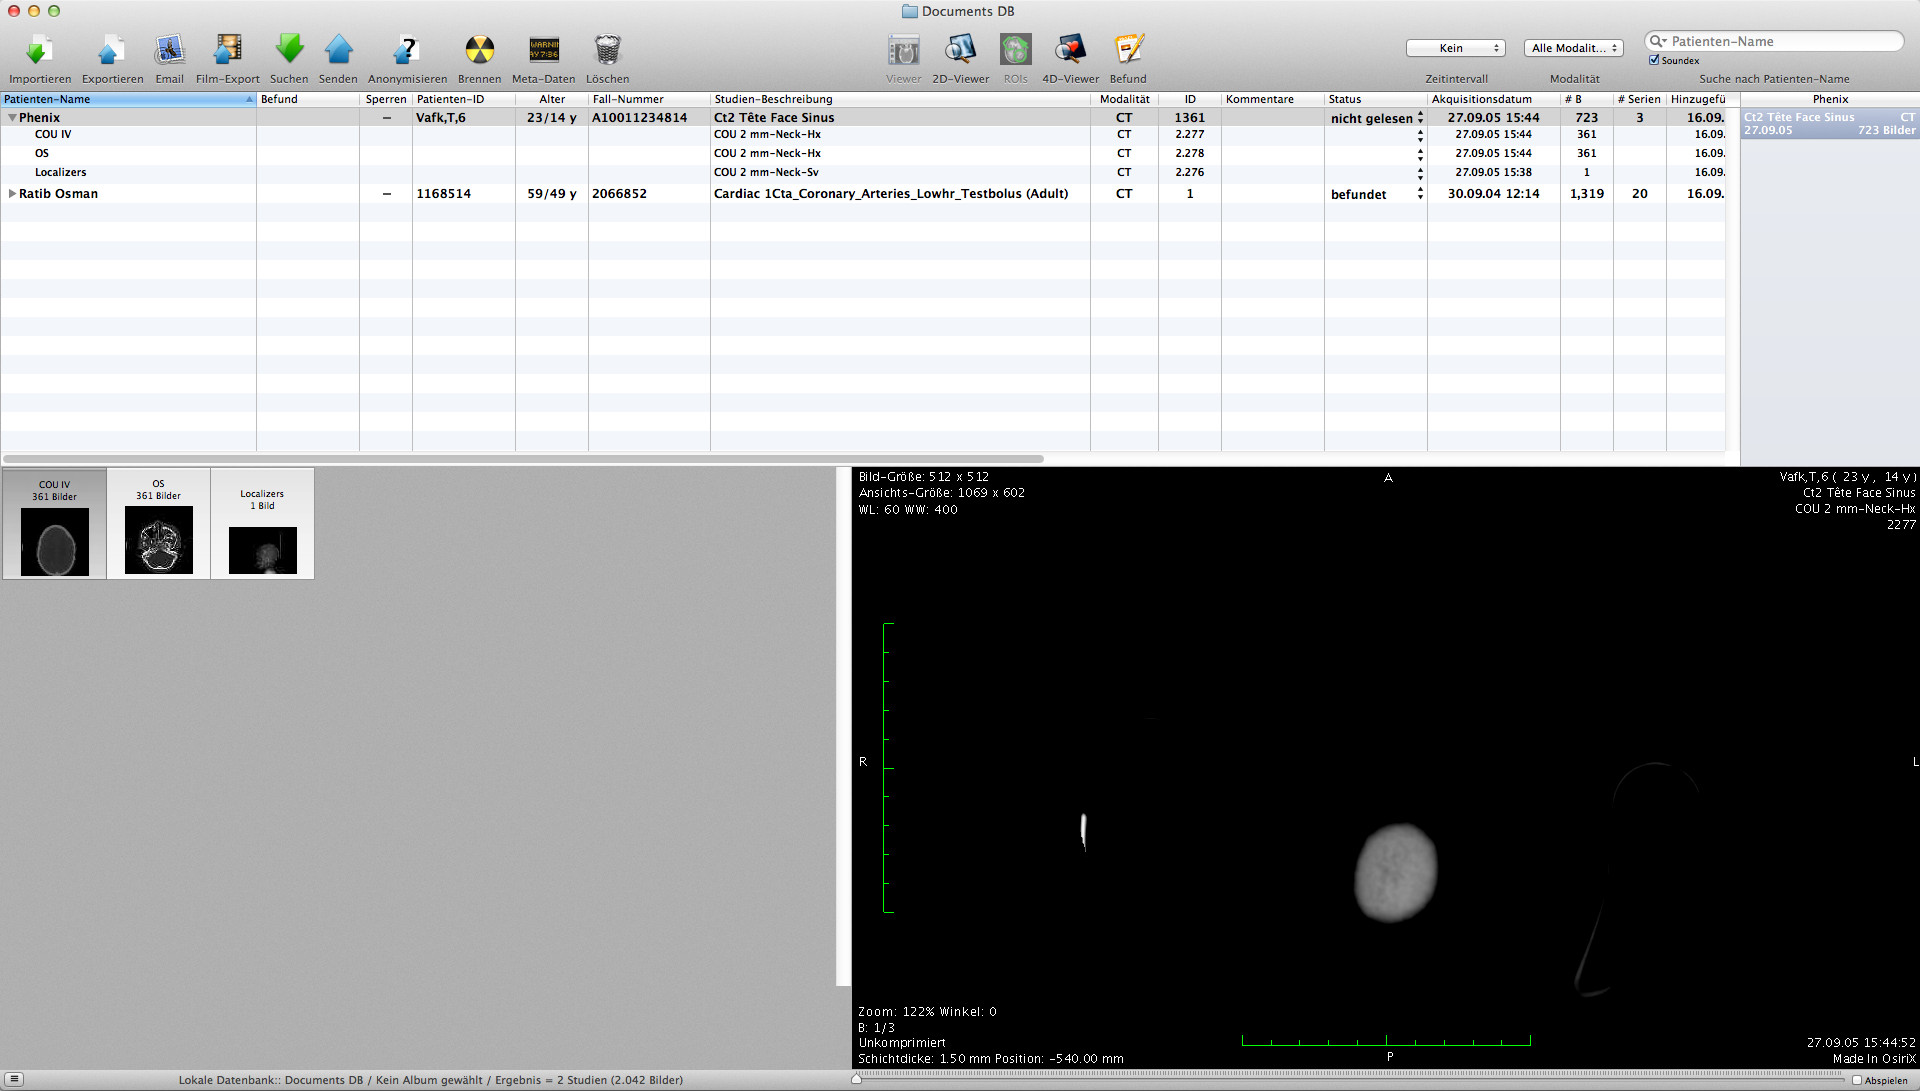
\includegraphics[width=0.8\linewidth]{img/c2_osirix_db_view.jpg}
	\caption{Datenbankansicht von OsiriX.}
	\label{fig:osirix_db_view}
\end{figure}
In der Datenbankebene können die Datensätze importiert, exportiert und durchsucht werden, wobei jede Studie für einen Patienten einen Eintrag in der Liste darstellt.
Weiters stehen Unterlisten zum Anzeigen der Serien einer Studie zur Verfügung.
Unter der Listenansicht werden die ausgewählten Einträge als Thumbnails und in einem minimalen 2D Betrachter,
welche die wichtigsten Funktionen der Betrachtungsebene implementiert, zur Vorschau dargestellt.
In der Betrachtungsebene \ref{fig:osiri_2dView_toolbar} \ref{fig:osirix_2dView_splitWindow} finden sich die eigentlichen Funktionen und Tools welche für die Interaktion mit den Bildern notwendig sind.
Dafür bietet OsiriX eine große Funktionspalette, wobei hier nur auf die Kernfunktionalität eingegangen wird \cite{osirix}.
\paragraph{Funktionsumfang}
Die Steuerung für die Tools zur Interaktion mit dem Volume erfolgt mit der Maus, 
welcher die spezifischen Funktionen zugewiesen werden können. Die jeweils zugewiesene Funktion wird durch das Drücken der Maustaste aktiv.
\begin{itemize}
	\item Bei der \textbf{Fensterung} wird mit der X-Achse wird die Fensterbreite (Kontrast) und mit der Y-Achse das Fensterzentrum (Helligkeit) angepasst.
	\item \textbf{Positionierung} des Bildes innerhalb der Anzeigefläche. Geht das Bild über die Anzeigefläche hinaus wird dies durch einen farbige Linie an der jeweiligen Kante signalisiert.
	\item \textbf{Zoom} durch das Verschieben der Maus entlang einer Achse.
	\item \textbf{Rotation} um das Bildzentrum durch das Verschieben  der Maus entlang der X-Achse.
	\item \textbf{Navigation} durch das Volume. Die Achse in der die Maus nach einem Klick zuerst verschoben wird, wird für die Navigation gewählt, die andere bleibt inaktiv.
	\item Einzeichnen von \textbf{ROIs}. Hierbei werden Punkte, Linien, Polygone, Winkel und noch weitere Geometrien unterstützt. 
		Sind in dem Datensatz die notwendigen Informationen vorhanden erfolgt einen automatische Vermessung der ROIs.
\end{itemize}
\begin{figure}[t]
	\centering
	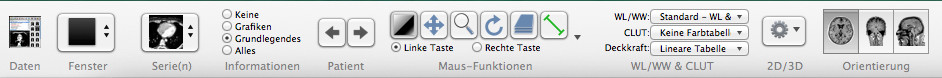
\includegraphics[width=0.8\linewidth]{img/c2_osirix_2d_view_toolbar.jpg}
	\caption{Toolbar für die 2D Batrachtungsebene.}
	\label{fig:osiri_2dView_toolbar}
\end{figure}
Weiters können mehrere Betrachtungs-Fenster nebeneinander angeordnet werden, wobei sich diese zur Darstellung unterschiedlicher Serien bzw. Orientierungen eines Datensatzes nutzen lassen. 
Die Orientierung gibt an entlang welcher Achse die Bilder eines Volumes geschnitten werden.
Wird in verschiedenen Fenstern eine unterschiedliche Orientierung gewählt,
so wird beim Navigieren durch das Volume in einem Fenster die Position der Schnittebene in den anderen als farbige Linie angezeigt \cite{osirix}.
\begin{figure}[t]
	\centering
	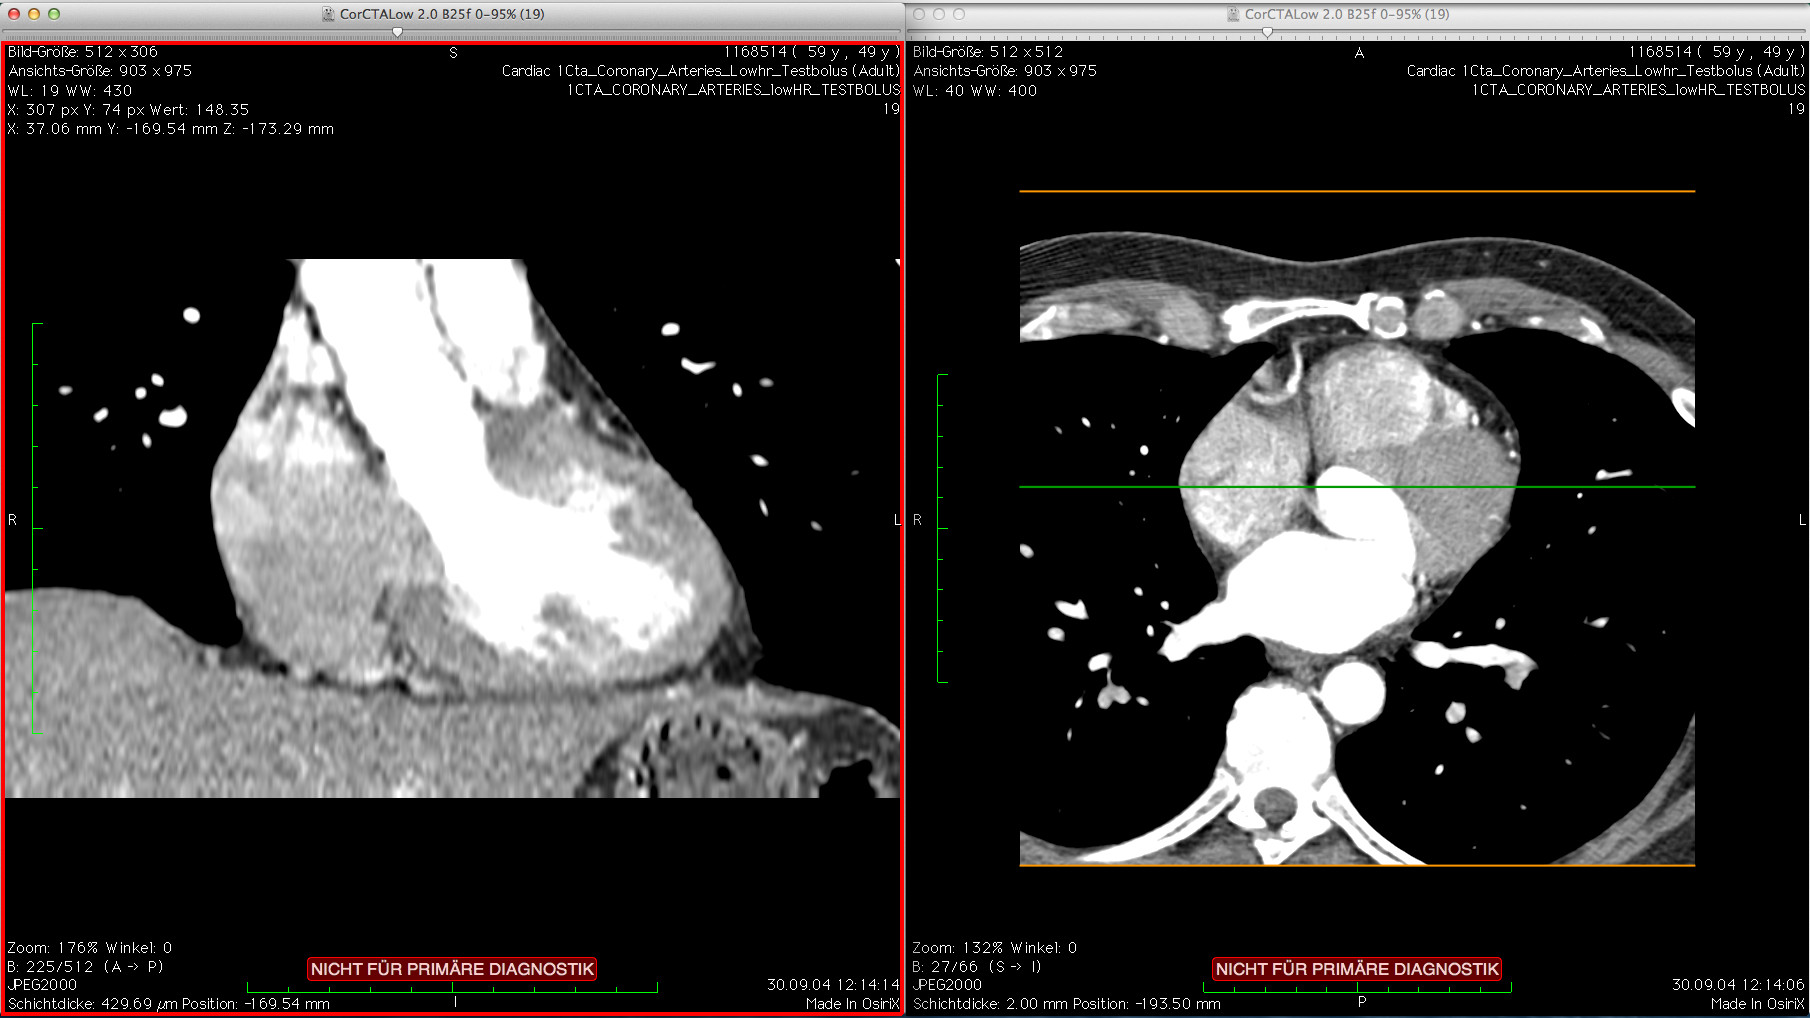
\includegraphics[width=0.8\linewidth]{img/c2_osirix_2d_view_splitscreen.jpg}
	\caption{Darstellung eines Volumes aus zwei verschiedenen Orientrierungen. Die Schnittposition des linken Bildes wird im rechten als grüne Linie dargestellt.}
	\label{fig:osirix_2dView_splitWindow}
\end{figure}

%----------------------------------------------
% * 
%----------------------------------------------
\subsection{XYZ - PACS Workstation}
\label{sec:XYZ - PACS Workstation}

%Abschließend angeben dass die Bildsuche bei keinen dieser systeme möglich ist


%TODO: Kontakt markus .... was gibst schon
%TODO: Kontakt markus .... pacs workstations

